\section{W11-12: Network Layer}
\textbf{Network address translation (NAT):} allows multiple devices to share a single public IP address.\\
\textbf{Subnets:} a network inside a network.\\
\textbf{Fragmentation:} breaking up packets into smaller packets.\\
\textbf{Transparent fragmentation:} routers can fragment packets.\\
\textbf{Nontransparent fragmentation:} only source router can fragment packets. This is used by IP.\\
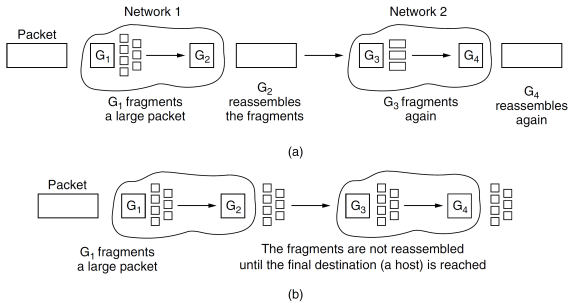
\includegraphics[width=\linewidth]{figs/fragmentation.png}\\

\subsection{Forwarding, routing}
\textbf{Packet forwarding:} each router has a forwarding table that maps destination addresses to outgoing interfaces. Get the destination address from the packet header and look it up in the forwarding table.\\
\textbf{Routing:} Routing algorithms are used to populate the forwarding tables.\\

\subsection{Routing within networks/domains}
\textbf{Non-adaptive routing:} routing tables are fixed.\\
\textbf{Adaptive routing:} routing tables change over time. Changes based on topology and potentially even traffic levels.\\
\textbf{Flooding:} send packet to all neighbors except the one it came from. Guarantees shortest distance, highly inefficient by generating duplicate packets, need to have a way of discarding duplicate packets (using TTL).\\
\textbf{Sink tree:} a tree that connects all sources to a single sink. Based on the optimality principle, the sink tree is the shortest path tree.\\
\textbf{Dijkstra's algorithm:} find the shortest path tree.\\
\begin{itemize}
    \item Divide nodes into three sets: \textit{unseen}, \textit{open} (tentative), \textit{closed} (permanent).
    \item Moves nodes from \textit{unseen} to \textit{open} to \textit{closed}.
    \item Initially, no paths are known, so all nodes are in \textit{unseen}.
    \item Set distance to source to 0 for source node, $\infty$ for all other nodes.
\end{itemize}
\begin{enumerate}
    \item Select node $n$ in \textit{open} with smallest distance to source.
    \item Move $n$ to \textit{closed}.
    \item For each neighbor $m$ of $n$ that is in \textit{unseen}, calculate distance from source to $m$ via $n$. If this distance is smaller than the current distance to $m$, update the distance to $m$ and set $n$ as the predecessor of $m$.
    \item Repeat until all nodes are in \textit{closed}.
\end{enumerate}
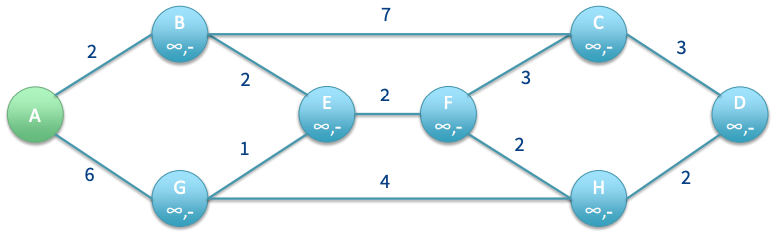
\includegraphics[width=\linewidth]{figs/dijkstra-example-1.png}\\
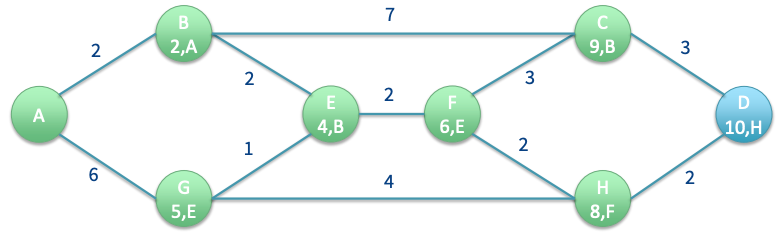
\includegraphics[width=\linewidth]{figs/dijkstra-example-2.png}\\

\subsection{Link state routing}
Variants of LS routing are used in practice. Simple 5 step process at each router:
\begin{enumerate}
    \item Discover neighbors and learn their network addresses.
    \item Measure the delay or cost to each neighbor.
    \item Construct a packet telling all you have just learned.
    \item Send this packet to, and receive packets from, all other routers.
    \item Compute the shortest path to every other router.
\end{enumerate}
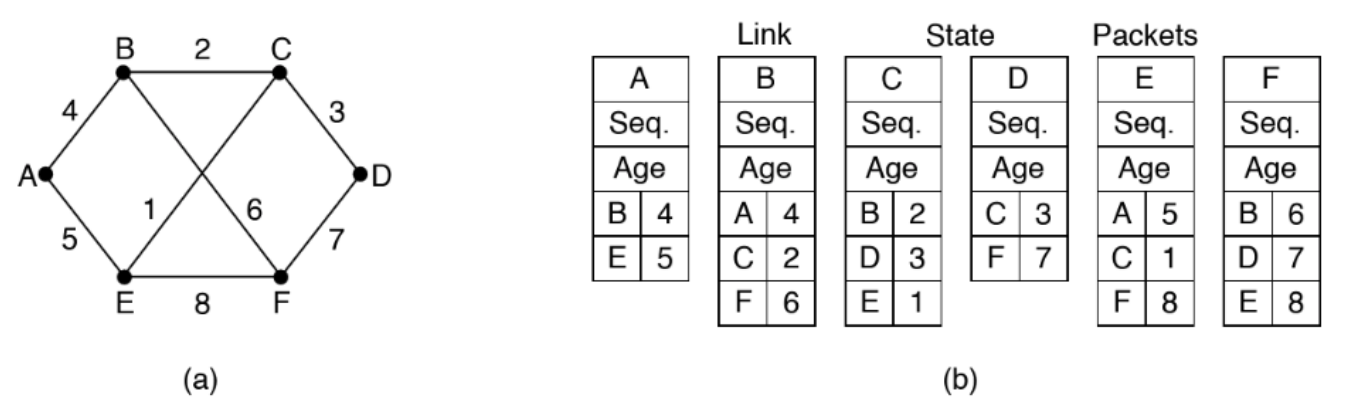
\includegraphics[width=\linewidth]{figs/link-state-packets.png}\\

\subsection{Interdomain routing (BGP)}
\textbf{Autonomous system (AS):} a network or group of networks under a single administrative authority.\\
\textbf{Border gateway protocol (BGP):} the routing protocol used between ASes.\\
\textbf{Politics:} Bellman's optimality principle doesn't always apply for interdomain routing.\\
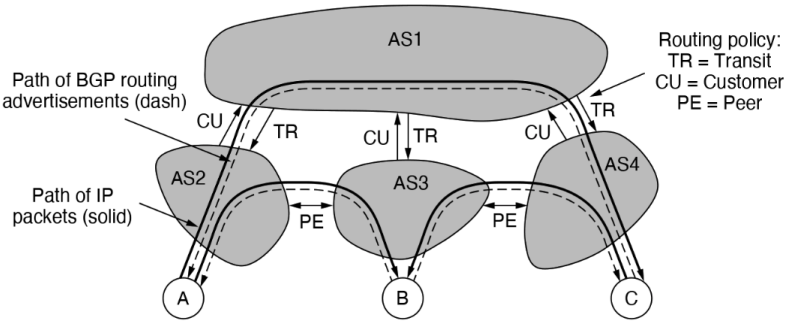
\includegraphics[width=\linewidth]{figs/bgp.png}\\

\subsection{Internet control protocols}
\textbf{Data plane (forwarding):} determines how packets are forwarded.\\
\textbf{Control plane (routing):} determines how routers communicate with each other.\\
\textbf{Internet control message protocol (ICMP):} used by routers and hosts to communicate network-level information.\\
\textbf{Traceroute:} uses ICMP to discover the path from a source to a destination. Exploits the Time Exceeded message in ICMP.\\
\begin{itemize}
    \item Send a packet with TTL = 1. The first router decrements TTL to 0, discards the packet, and sends an ICMP Time Exceeded message back to the source.
    \item Send a packet with TTL = 2. The first router decrements TTL to 1, forwards the packet to the second router, which decrements TTL to 0, discards the packet, and sends an ICMP Time Exceeded message back to the source.
    \item Repeat until the packet reaches the destination.
\end{itemize}

\textbf{Dynamic host configuration protocol (DHCP):} used by hosts to send out a DHCP DISCOVER packet, to obtain IP addresses from a DHCP server mediated through a DHCP OFFER packet. We use MAC addresses to identify hosts.\\

\textbf{Address Resolution Protocol (ARP):} used by hosts to discover the MAC address of a host given its IP address. ARP will broadcast a packet asking who owns the target IP address. The broadcast arrives at every host on the network, but only the host with the target IP address will respond. ARP spoofing is the gateway attack for most MITM attacks.\\
